% ARMS: A Spatial Memory Fabric for AI Systems
% arXiv submission - January 2026

\documentclass[11pt,a4paper]{article}

% ============================================================================
% PACKAGES
% ============================================================================

\usepackage[utf8]{inputenc}
\usepackage[T1]{fontenc}
\usepackage{lmodern}

% Math
\usepackage{amsmath,amssymb,amsthm}
\usepackage{mathtools}

% Graphics
\usepackage{graphicx}
\usepackage{float}
\usepackage{subcaption}
\usepackage[dvipsnames]{xcolor}
\graphicspath{{figures/}{Diagrams/}}

% Tables
\usepackage{booktabs}
\usepackage{multirow}
\usepackage{array}

% Algorithms
\usepackage{algorithm}
\usepackage{algorithmic}

% Code
\usepackage{listings}
\lstset{
    basicstyle=\ttfamily\small,
    breaklines=true,
    frame=single,
    numbers=left,
    numberstyle=\tiny,
    language=Python,
}

% Links
\usepackage[colorlinks=true,linkcolor=blue,citecolor=blue,urlcolor=blue]{hyperref}
\usepackage{cleveref}

% Layout
\usepackage[margin=1in]{geometry}

% Bibliography
\usepackage[numbers,sort&compress]{natbib}

% ============================================================================
% CUSTOM COMMANDS
% ============================================================================

\DeclareMathOperator*{\argmax}{arg\,max}
\DeclareMathOperator*{\argmin}{arg\,min}
\newcommand{\R}{\mathbb{R}}

% ============================================================================
% TITLE
% ============================================================================

\title{%
    \textbf{ARMS: A Spatial Memory Fabric for AI Systems}\\[0.5em]
    \large Position IS Relationship
}

\author{%
    Andrew Young\\
    \texttt{andrew@automate-capture.com}
}

\date{January 2026}

% ============================================================================
% DOCUMENT
% ============================================================================

\begin{document}

\maketitle

% ----------------------------------------------------------------------------
\begin{abstract}
\noindent
This paper introduces ARMS (Attention Reasoning Memory Store), a spatial memory fabric that enables AI systems to store and retrieve computed states by their native dimensional coordinates. Unlike traditional databases that require explicit relationships through foreign keys or learned topology through approximate nearest neighbor algorithms, ARMS operates on a fundamental principle: \textbf{position IS relationship}. Proximity in high-dimensional space defines semantic connection without explicit declaration.

ARMS reduces memory operations to five primitives: \textbf{Point} (any-dimensional vectors), \textbf{Proximity} (relationship measurement), \textbf{Merge} (composition), \textbf{Place} (existence in space), and \textbf{Near} (retrieval by similarity). This minimal abstraction enables a hexagonal architecture where storage backends, index algorithms, and APIs can be swapped without changing core logic.

The framework provides the foundation for specialized index adapters like HAT (Hierarchical Attention Tree), demonstrating that domain-specific structure can be exploited for superior performance. ARMS functions as an artificial hippocampus---enabling AI systems to form, consolidate, and retrieve episodic memories through spatial organization rather than explicit indexing.

\vspace{1em}
\noindent\textbf{Keywords:} spatial memory, AI memory systems, vector databases, hexagonal architecture, episodic memory
\end{abstract}

% ----------------------------------------------------------------------------
\section{Introduction}
\label{sec:intro}

\subsection{The Memory Problem in AI}

Large language models and AI agents face a fundamental limitation: they lack persistent, retrievable memory beyond their context window. Current approaches include:

\begin{itemize}
    \item \textbf{Extended context}: Expensive, doesn't scale beyond training length
    \item \textbf{RAG retrieval}: Retrieves text, requires recomputation of attention
    \item \textbf{Vector databases}: Treat all data as unstructured point clouds
    \item \textbf{External memory}: Key-value stores with explicit indexing
\end{itemize}

None of these approaches preserve the \emph{native representation} of computed states. When an LLM processes text, it produces attention states in high-dimensional space. Current systems project, compress, or discard these states rather than storing them directly.

\begin{figure}[H]
\centering
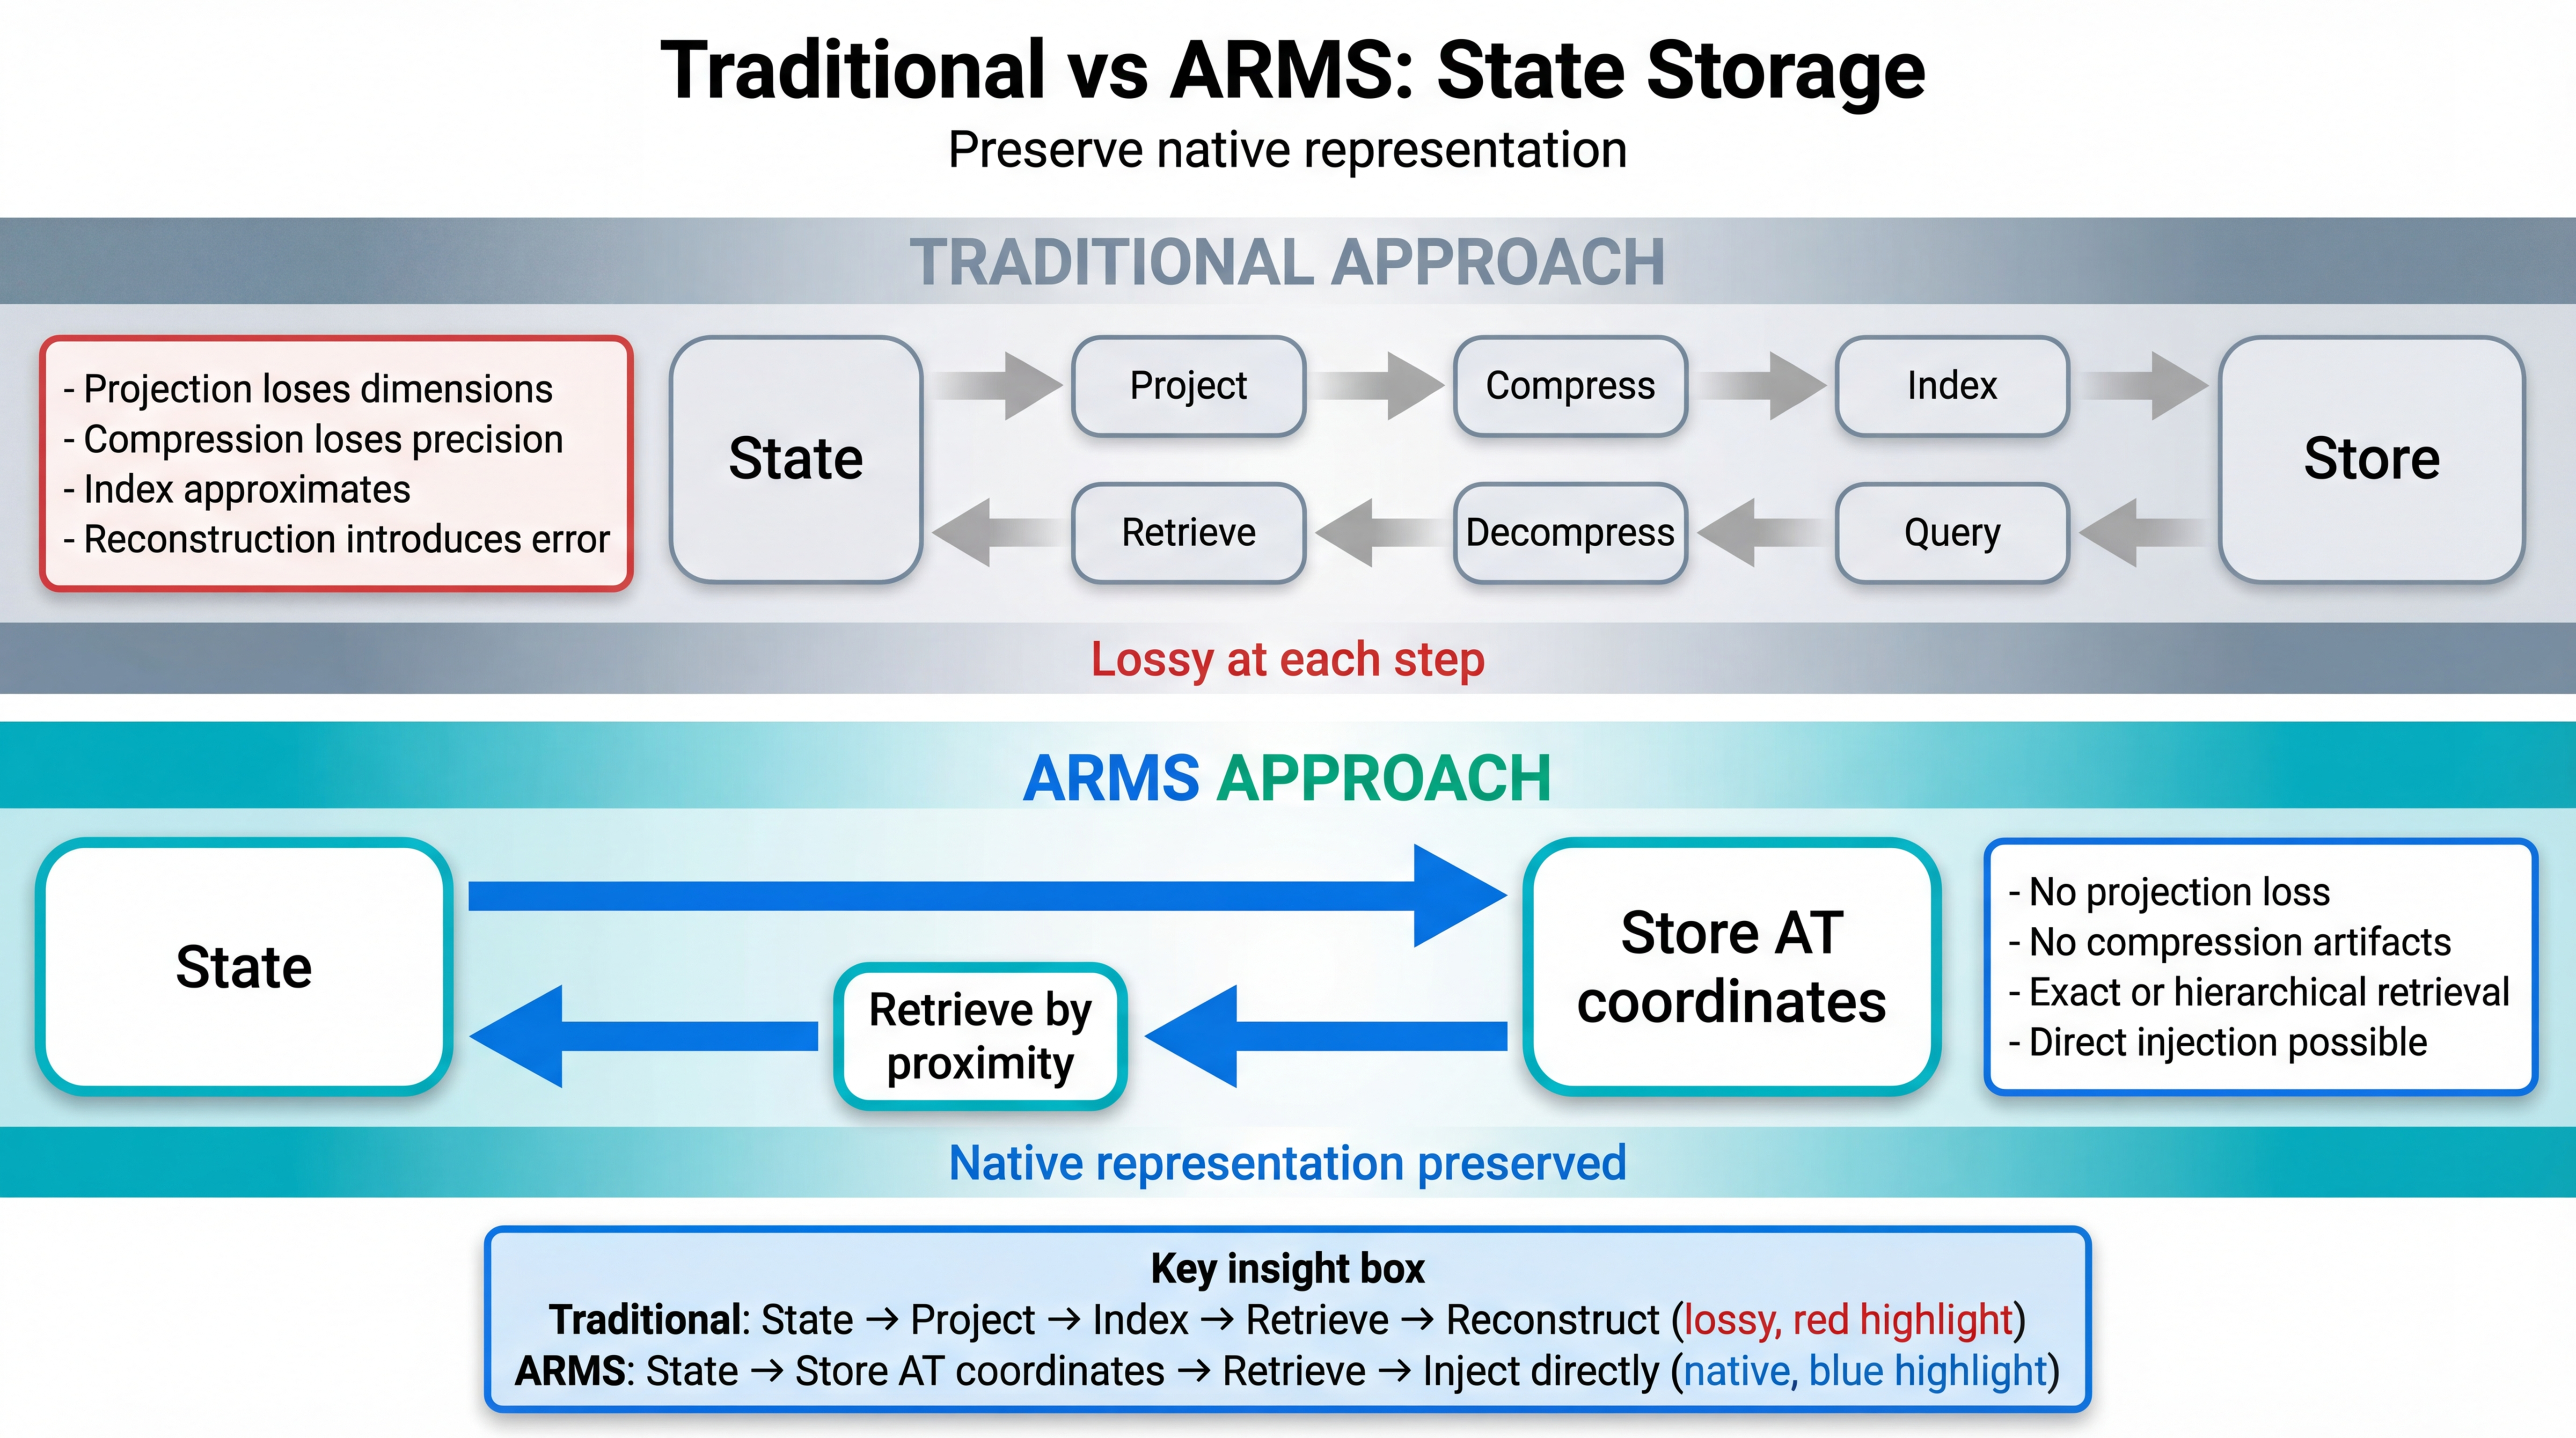
\includegraphics[width=0.9\textwidth]{fig06_traditional_vs_arms.jpg}
\caption{Traditional approaches vs ARMS: Traditional systems project, compress, and approximate states at each step, introducing cumulative error. ARMS stores states at their native coordinates and retrieves by proximity, preserving the original representation.}
\label{fig:traditional}
\end{figure}

\subsection{The ARMS Insight}

ARMS takes a different approach:

\begin{quote}
\textbf{Store states at their native coordinates. Retrieve by proximity. Position IS relationship.}
\end{quote}

This insight has three implications:

\begin{enumerate}
    \item \textbf{No projection loss}: States are stored in their original dimensionality
    \item \textbf{No explicit relationships}: Semantic similarity is spatial proximity
    \item \textbf{No learned topology}: Structure can be known or exploited, not discovered
\end{enumerate}

\begin{figure}[H]
\centering
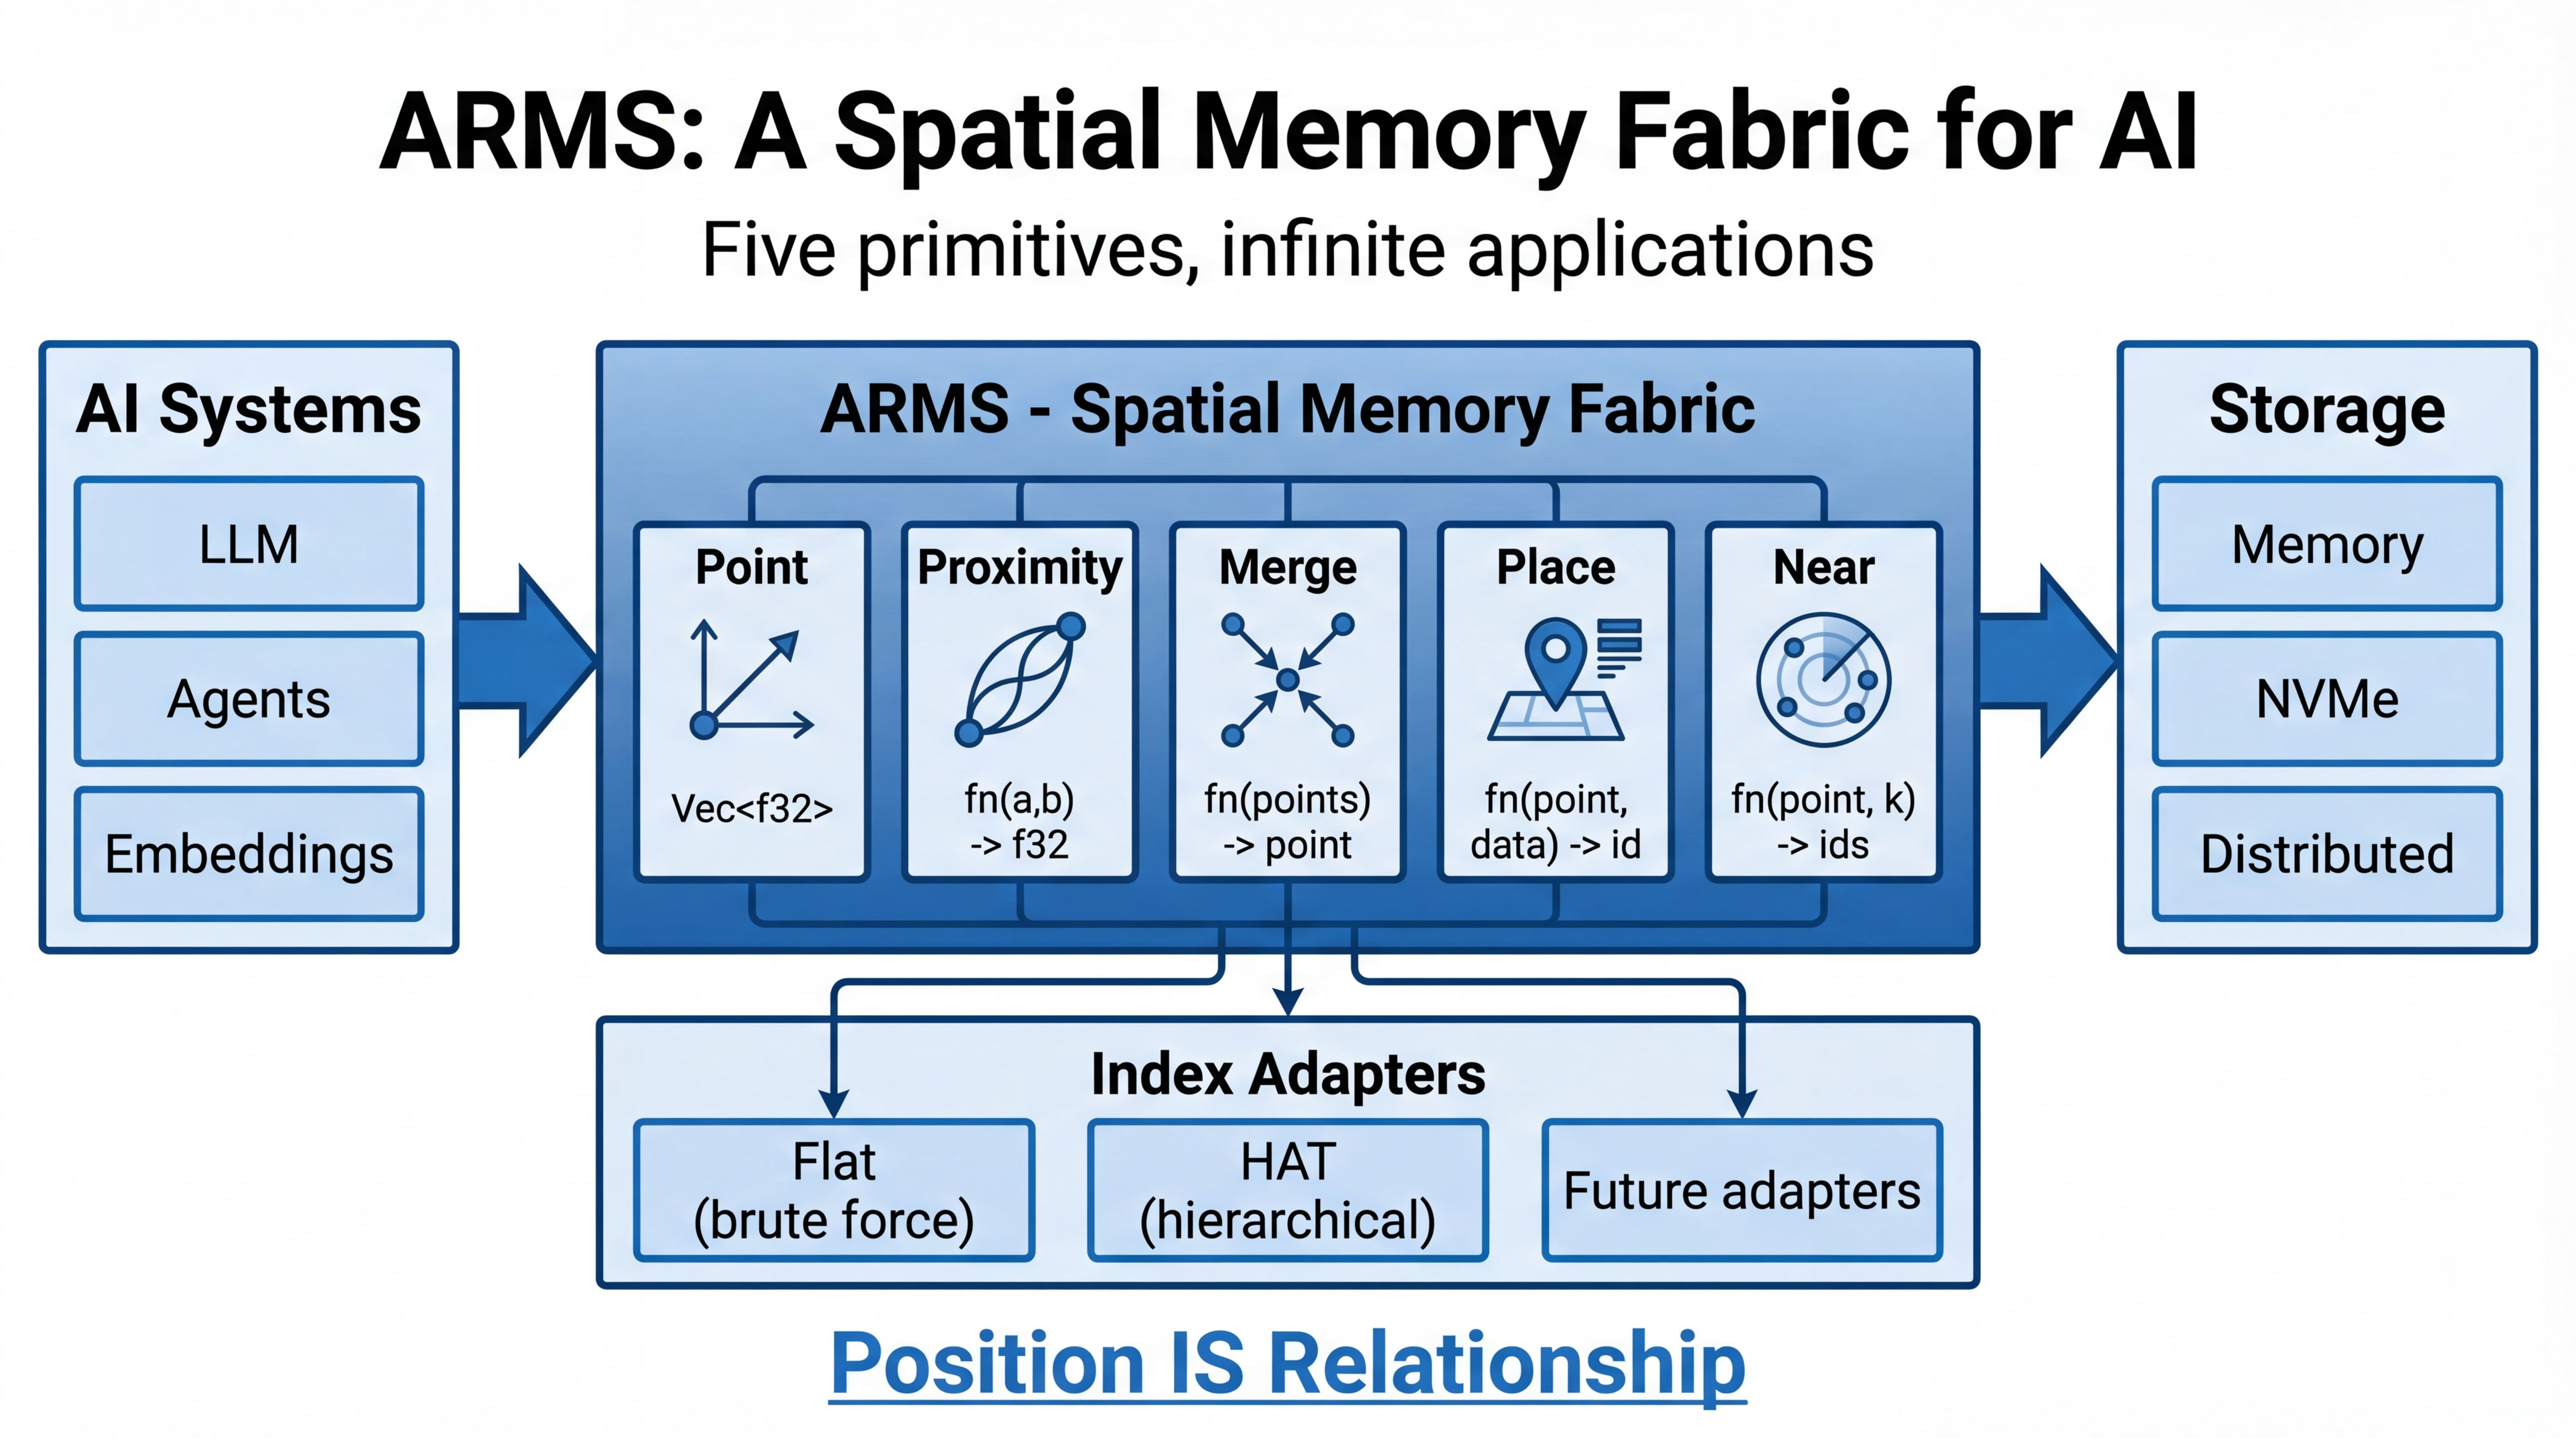
\includegraphics[width=0.9\textwidth]{fig01_architecture.jpg}
\caption{ARMS architecture overview. The five primitives (Point, Proximity, Merge, Place, Near) form the core, with swappable storage and index adapters.}
\label{fig:architecture}
\end{figure}

\subsection{Contributions}

This paper makes the following contributions:

\begin{enumerate}
    \item A \textbf{five-primitive abstraction} for spatial memory (Point, Proximity, Merge, Place, Near)
    \item A \textbf{hexagonal architecture} enabling swappable storage, index, and API adapters
    \item The \textbf{``position is relationship''} principle for AI memory systems
    \item A \textbf{foundation framework} demonstrated through the HAT index adapter
\end{enumerate}

% ----------------------------------------------------------------------------
\section{The Five Primitives}
\label{sec:primitives}

ARMS reduces all memory operations to five primitives. This minimal surface area enables maximum flexibility while maintaining semantic clarity.

\begin{figure}[H]
\centering
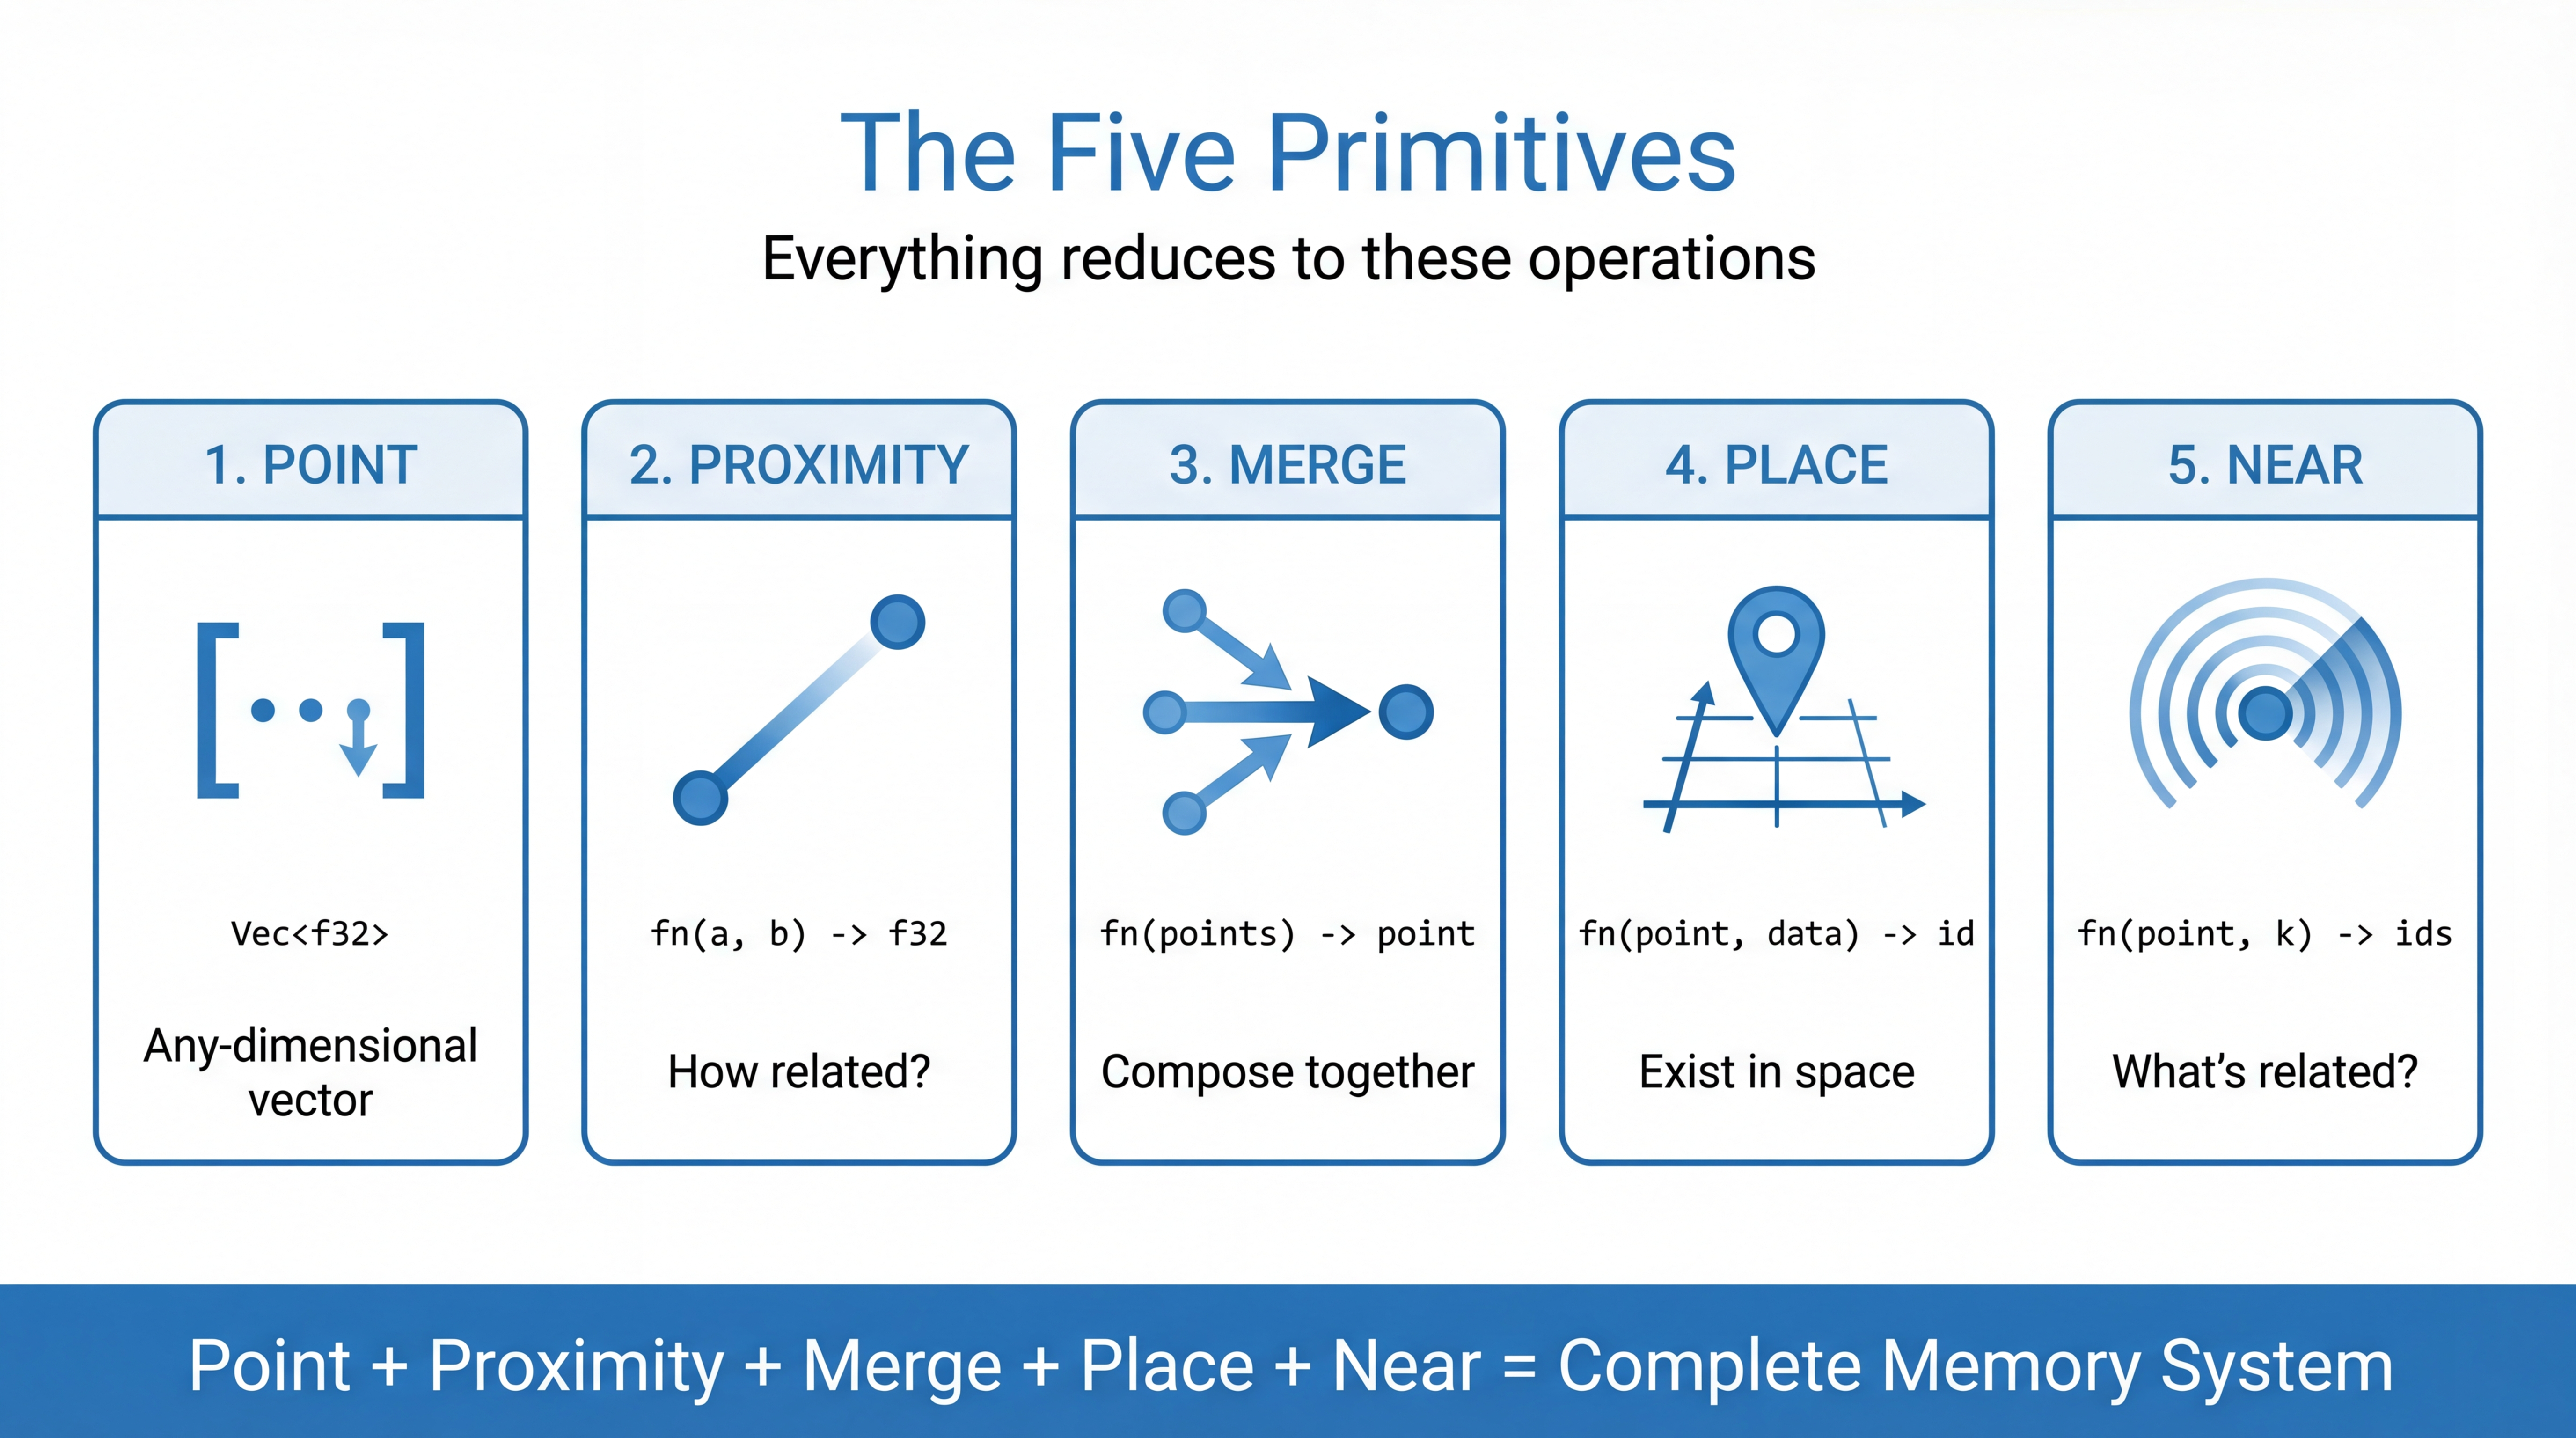
\includegraphics[width=0.85\textwidth]{fig03_primitives.jpg}
\caption{The five primitives of ARMS: Point (representation), Proximity (relationship), Merge (composition), Place (storage), and Near (retrieval). These operations form the complete interface for spatial memory.}
\label{fig:primitives}
\end{figure}

\begin{table}[H]
\centering
\caption{The five primitives of ARMS.}
\label{tab:primitives}
\begin{tabular}{llp{7cm}}
\toprule
\textbf{Primitive} & \textbf{Signature} & \textbf{Purpose} \\
\midrule
Point & \texttt{Vec<f32>} & Any-dimensional vector representation \\
Proximity & \texttt{fn(a, b) -> f32} & Measure how related two points are \\
Merge & \texttt{fn(points) -> point} & Compose multiple points into one \\
Place & \texttt{fn(point, data) -> id} & Store a point in the space \\
Near & \texttt{fn(point, k) -> ids} & Find k most related points \\
\bottomrule
\end{tabular}
\end{table}

\subsection{Point: The Universal Representation}

A Point is simply a vector of floating-point numbers:

\begin{lstlisting}[language=Rust,caption={Point definition.}]
pub struct Point {
    dims: Vec<f32>,
}

impl Point {
    pub fn new(dims: Vec<f32>) -> Self;
    pub fn dimensionality(&self) -> usize;
    pub fn magnitude(&self) -> f32;
    pub fn normalize(&self) -> Point;
}
\end{lstlisting}

Points are dimensionality-agnostic. The same ARMS instance can store 768-dimensional BERT embeddings or 1536-dimensional OpenAI embeddings---the primitives don't change.

\subsection{Proximity: Relationship Without Declaration}

Proximity functions measure how related two points are:

\begin{table}[H]
\centering
\caption{Built-in proximity functions.}
\label{tab:proximity}
\begin{tabular}{llp{6cm}}
\toprule
\textbf{Function} & \textbf{Range} & \textbf{Use Case} \\
\midrule
Cosine & $[-1, 1]$ & Semantic similarity (direction matters) \\
Euclidean & $[0, \infty)$ & Spatial distance (magnitude matters) \\
DotProduct & $(-\infty, \infty)$ & Raw correlation \\
Manhattan & $[0, \infty)$ & L1 distance \\
\bottomrule
\end{tabular}
\end{table}

The key insight: \textbf{proximity replaces foreign keys}. In a relational database, you declare relationships explicitly. In ARMS, relationships emerge from spatial position.

\subsection{Merge: Composition Without Loss}

Merge combines multiple points into a single representative:

\begin{itemize}
    \item \textbf{Mean}: Arithmetic average (default)
    \item \textbf{WeightedMean}: Importance-weighted average
    \item \textbf{MaxPool}: Element-wise maximum
\end{itemize}

Merge enables hierarchical summarization. A conversation can be represented by the merge of its messages; a session by the merge of its conversations.

\subsection{Place and Near: The Memory Interface}

Place stores a point with associated data:

\begin{lstlisting}[language=Rust,caption={Place and Near operations.}]
// Store
let id = arms.place(embedding, blob)?;

// Retrieve
let neighbors = arms.near(&query, k)?;
\end{lstlisting}

This is the complete memory interface. Everything else---storage backends, index algorithms, APIs---is implementation detail.

% ----------------------------------------------------------------------------
\section{Hexagonal Architecture}
\label{sec:architecture}

ARMS follows hexagonal (ports-and-adapters) architecture. The core domain contains pure math with no I/O. Ports define trait contracts. Adapters provide swappable implementations.

\begin{figure}[H]
\centering
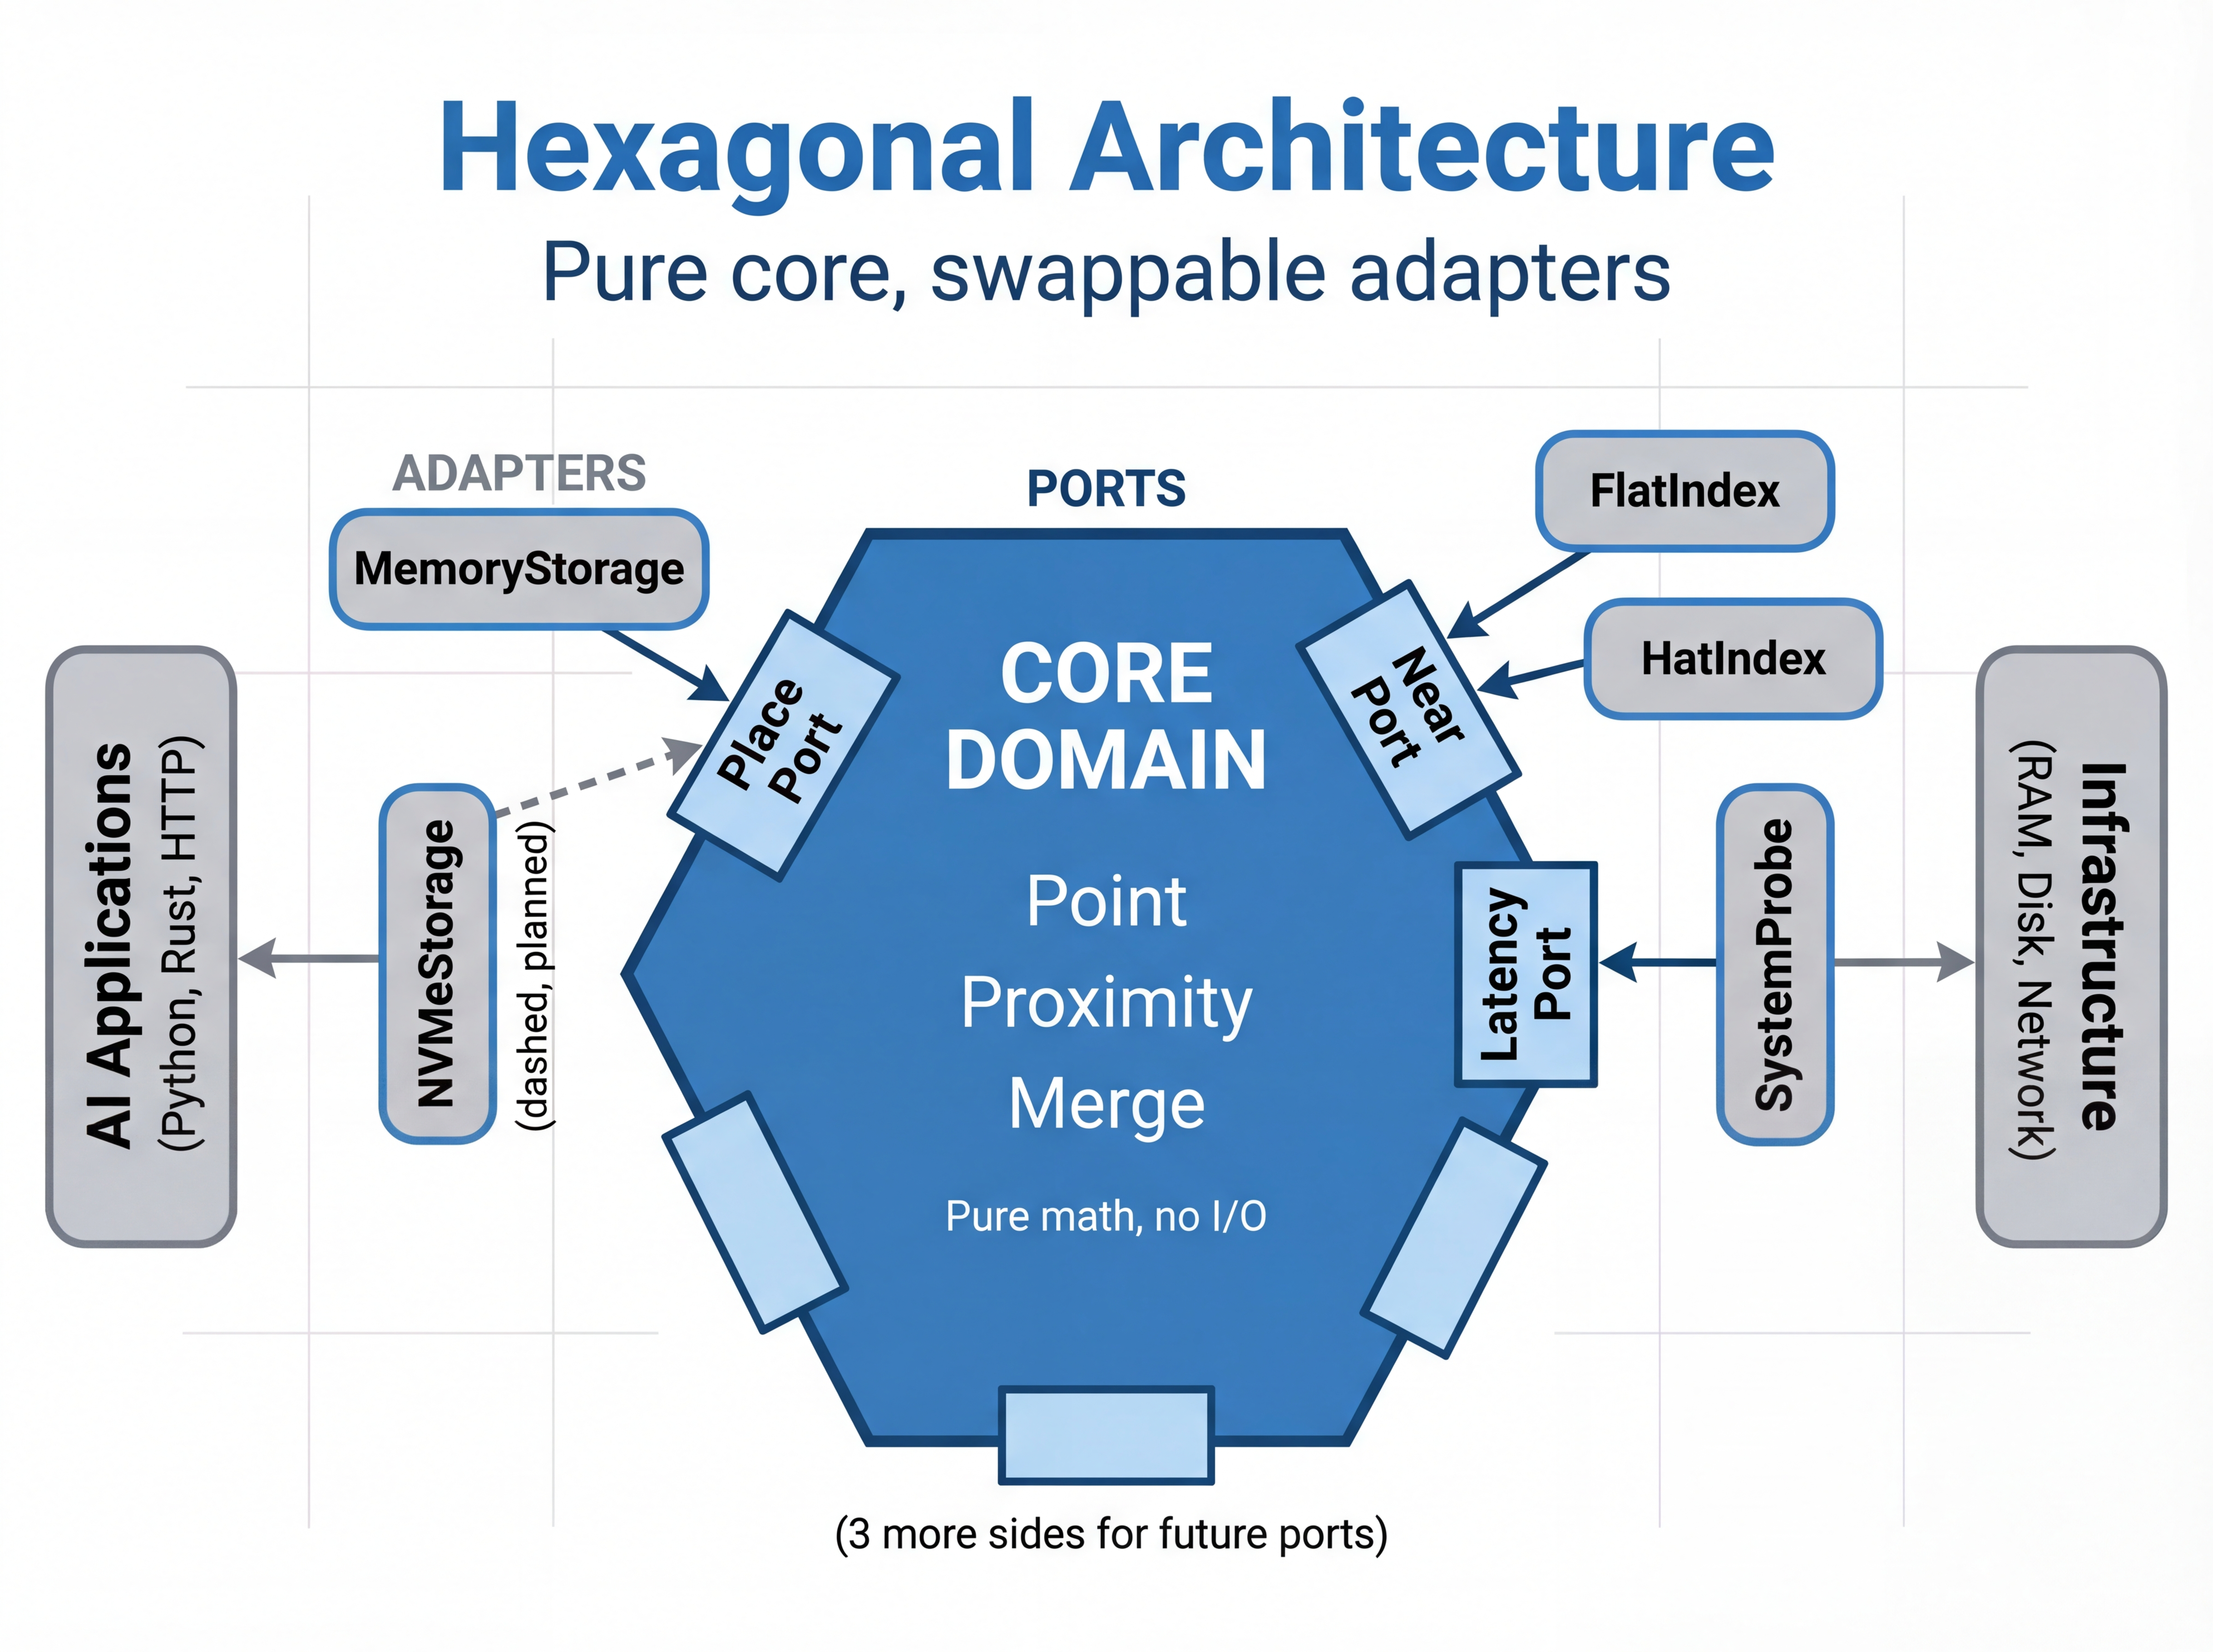
\includegraphics[width=0.9\textwidth]{fig02_hexagonal.jpg}
\caption{Hexagonal architecture of ARMS. The core domain contains pure math with no I/O. Ports define trait contracts. Adapters provide swappable implementations for storage, indexing, and APIs.}
\label{fig:hexagonal}
\end{figure}

\subsection{Core Domain}

The core contains:

\begin{itemize}
    \item \textbf{Point}: Vector representation
    \item \textbf{Id}: Unique identifiers
    \item \textbf{Blob}: Associated data
    \item \textbf{Proximity}: Relationship measurement
    \item \textbf{Merge}: Point composition
\end{itemize}

No I/O, no side effects, pure functions. This enables testing without mocks and reasoning without context.

\subsection{Ports}

Ports define what the system needs without specifying how:

\begin{lstlisting}[language=Rust,caption={Port definitions.}]
pub trait Place {
    fn place(&mut self, point: Point, blob: Blob) -> Result<Id>;
    fn get(&self, id: Id) -> Option<&PlacedPoint>;
    fn remove(&mut self, id: Id) -> Option<PlacedPoint>;
}

pub trait Near {
    fn near(&self, query: &Point, k: usize) -> Result<Vec<SearchResult>>;
    fn add(&mut self, id: Id, point: &Point) -> Result<()>;
}
\end{lstlisting}

\subsection{Adapters}

Adapters implement ports for specific technologies:

\begin{table}[H]
\centering
\caption{Available adapters.}
\label{tab:adapters}
\begin{tabular}{lll}
\toprule
\textbf{Port} & \textbf{Adapter} & \textbf{Description} \\
\midrule
Place & MemoryStorage & In-memory hash map \\
Place & NVMeStorage & Memory-mapped files (planned) \\
Near & FlatIndex & Brute-force exact search \\
Near & HatIndex & Hierarchical Attention Tree \\
\bottomrule
\end{tabular}
\end{table}

The HAT index adapter (published separately as \texttt{arms-hat}) demonstrates how domain-specific knowledge can be exploited for superior performance on hierarchical data.

\begin{figure}[H]
\centering
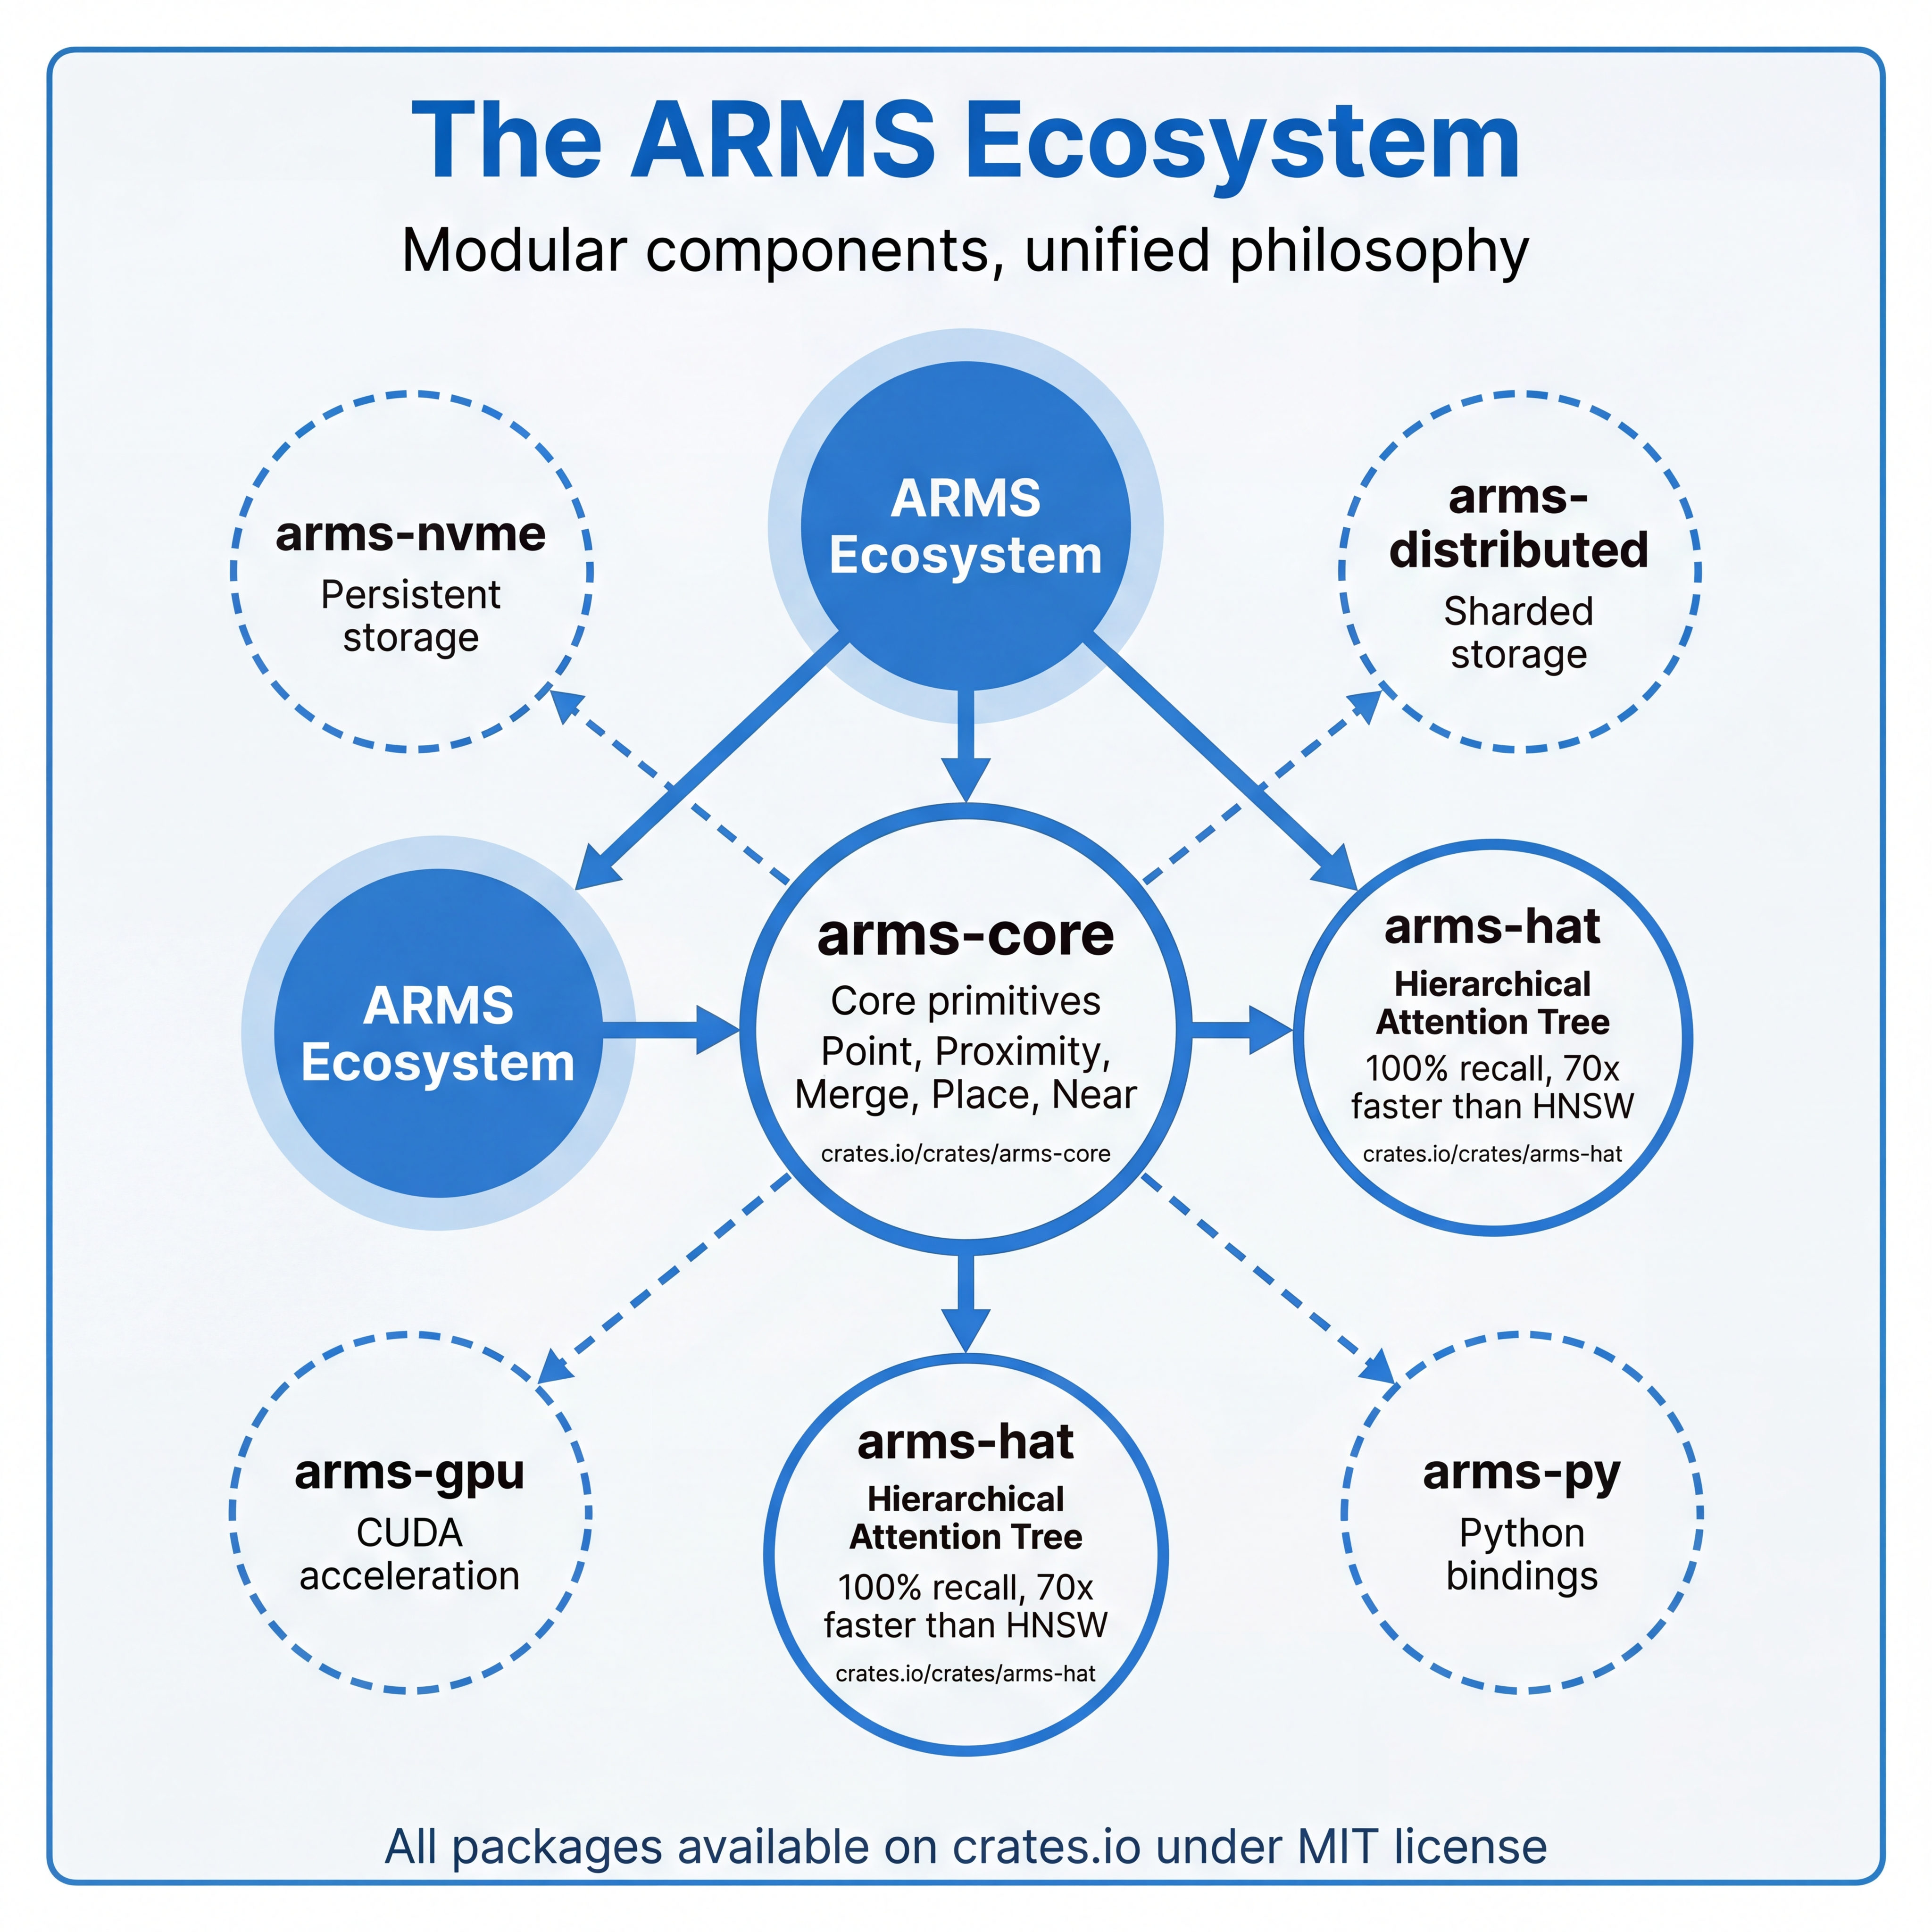
\includegraphics[width=0.85\textwidth]{fig07_ecosystem.jpg}
\caption{The ARMS ecosystem: \texttt{arms-core} provides the foundational primitives, while specialized adapters like \texttt{arms-hat} exploit domain-specific structure. Future adapters will add persistence, distribution, and GPU acceleration.}
\label{fig:ecosystem}
\end{figure}

% ----------------------------------------------------------------------------
\section{Position IS Relationship}
\label{sec:philosophy}

The core philosophical innovation of ARMS is treating position as the fundamental relationship primitive.

\begin{figure}[H]
\centering
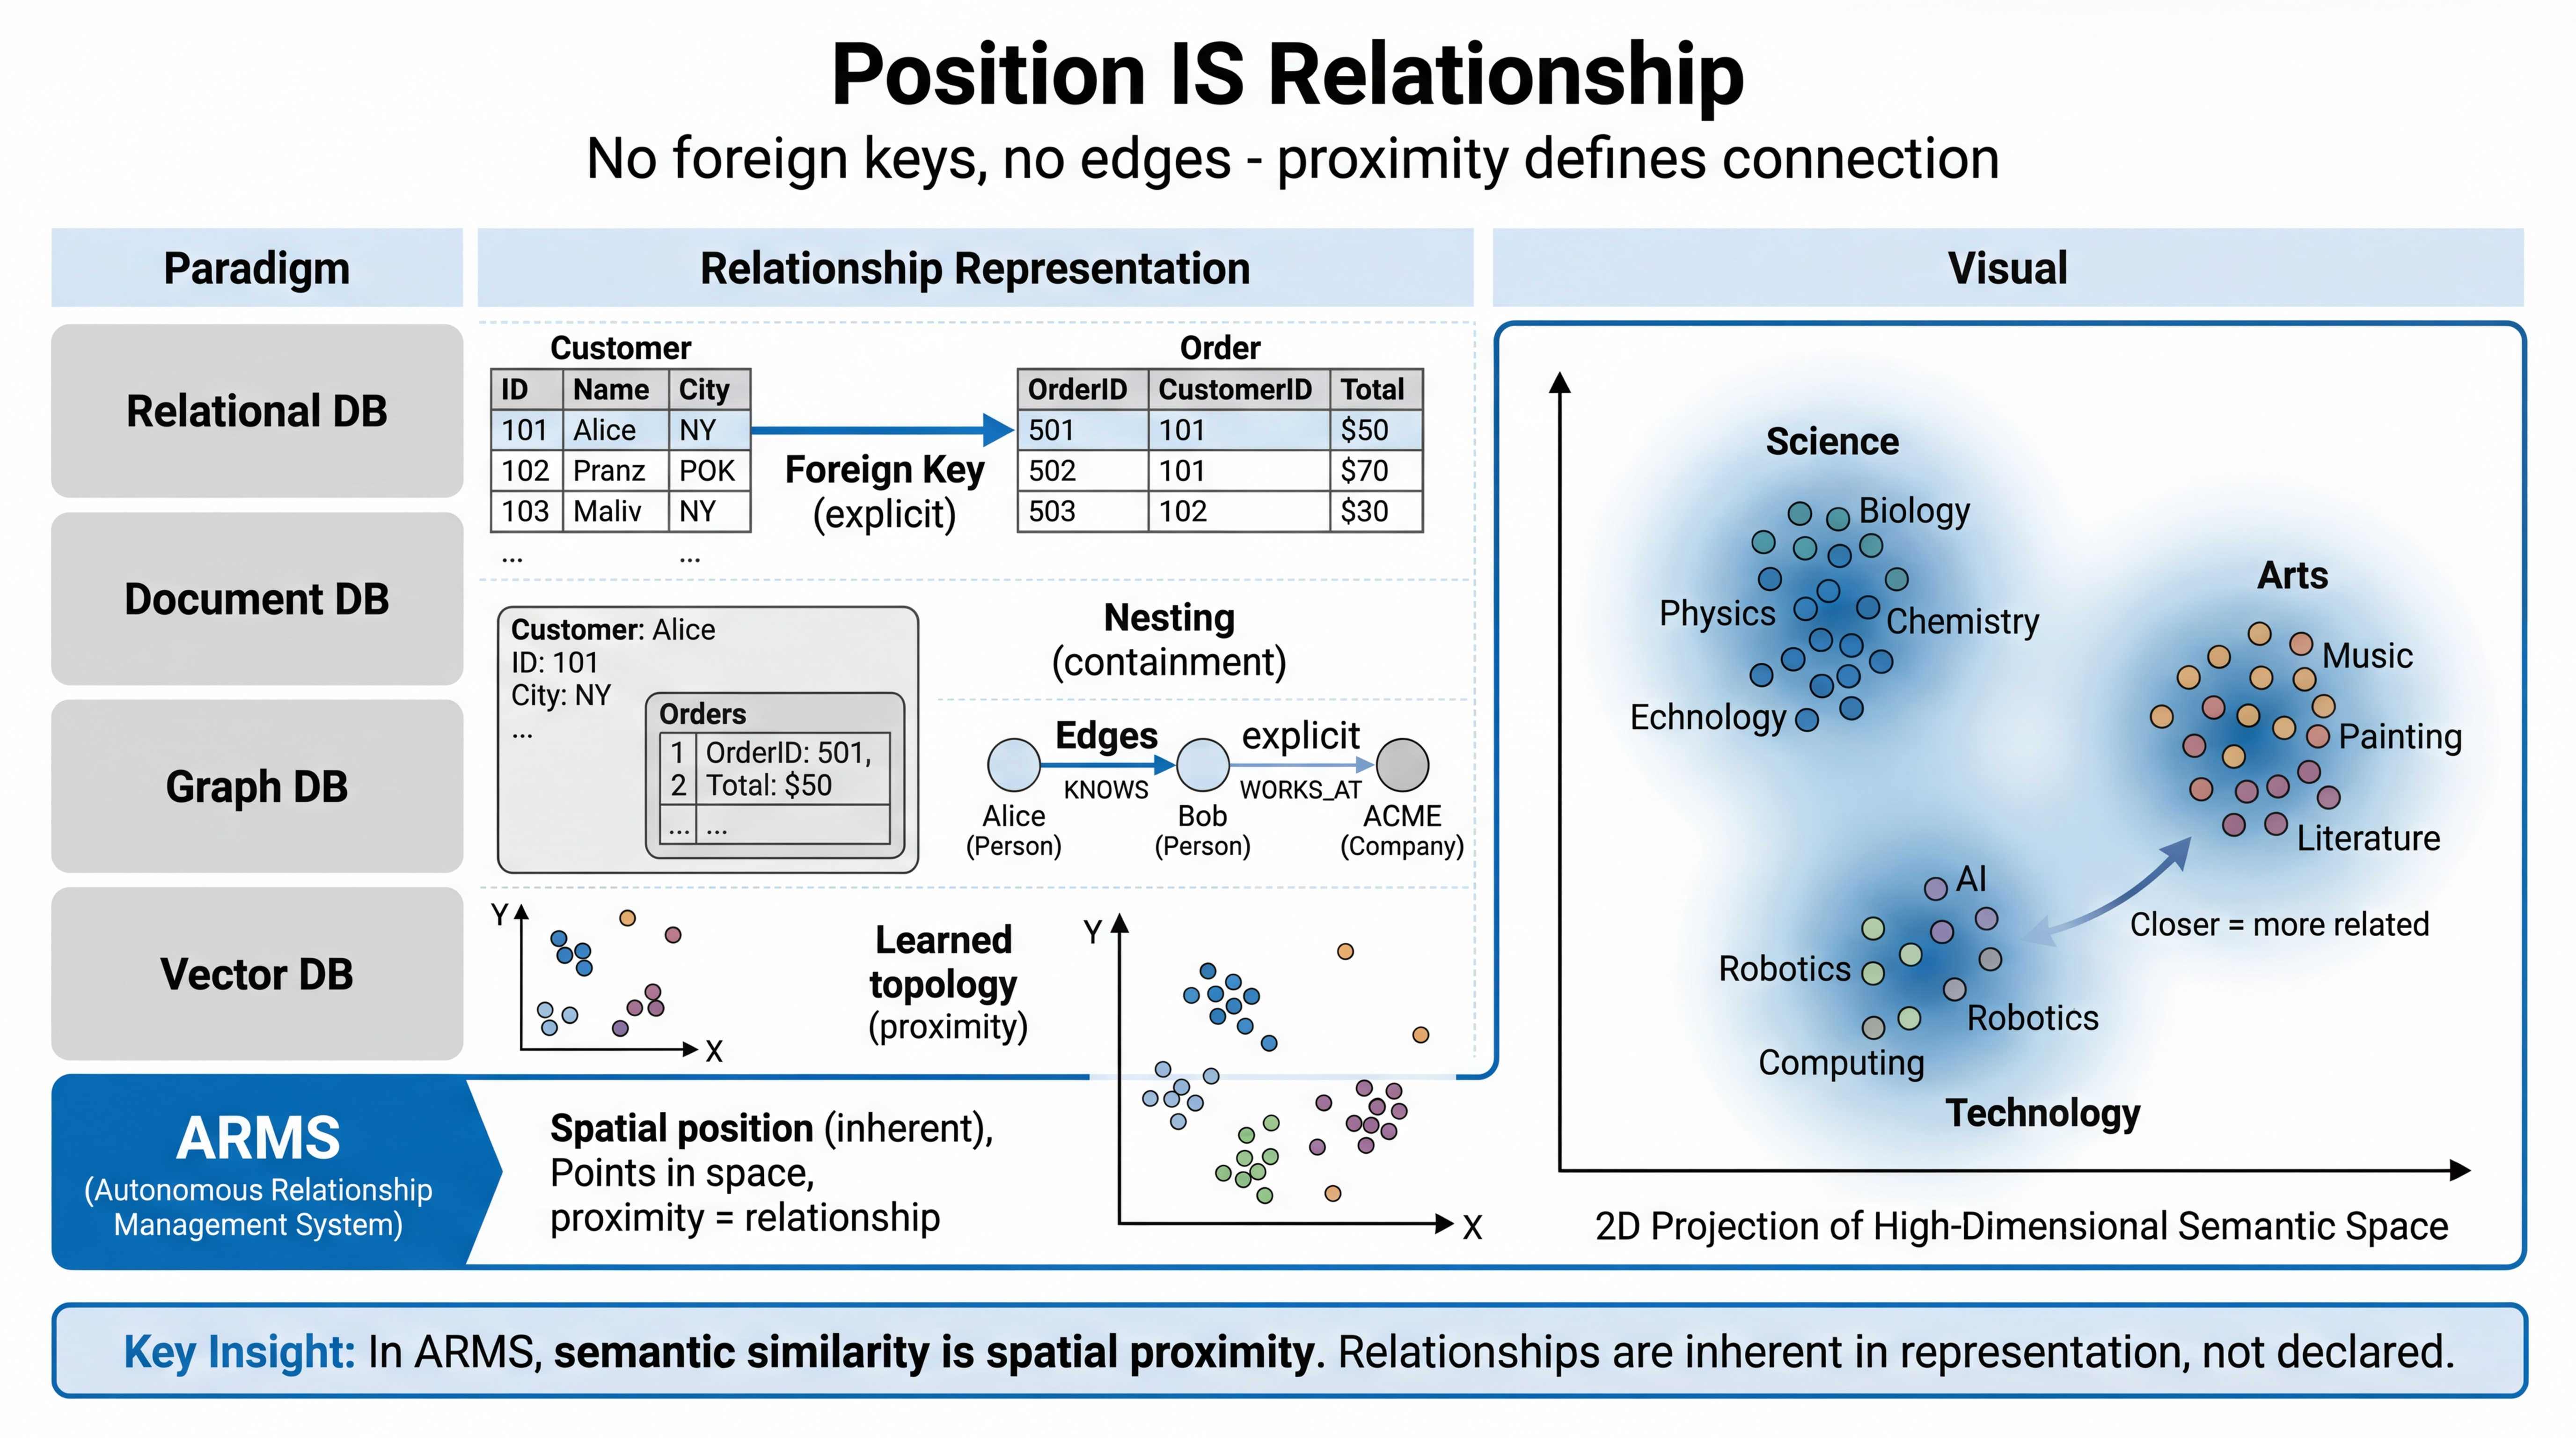
\includegraphics[width=0.9\textwidth]{fig04_position_relationship.jpg}
\caption{Position IS relationship: Comparison of relationship representation across database paradigms. ARMS uses spatial position as the fundamental relationship primitive, eliminating the need for explicit declarations.}
\label{fig:position}
\end{figure}

\subsection{Traditional Approaches}

\begin{table}[H]
\centering
\caption{Relationship representation in different paradigms.}
\label{tab:paradigms}
\begin{tabular}{lll}
\toprule
\textbf{Paradigm} & \textbf{Relationship} & \textbf{Limitation} \\
\midrule
Relational DB & Foreign keys & Must be declared explicitly \\
Document DB & Nesting & Limited to containment \\
Graph DB & Edges & Must be declared explicitly \\
Vector DB & Learned topology & Requires training/building \\
\textbf{ARMS} & \textbf{Spatial position} & \textbf{Inherent in representation} \\
\bottomrule
\end{tabular}
\end{table}

\subsection{Implications}

When position is relationship:

\begin{enumerate}
    \item \textbf{Schema-free}: No need to declare relationship types
    \item \textbf{Continuous}: Relationships have degrees, not just existence
    \item \textbf{Emergent}: New relationships discovered through proximity
    \item \textbf{Composable}: Merged points represent group relationships
\end{enumerate}

\subsection{The Hippocampus Analogy}

ARMS mirrors the function of the biological hippocampus:

\begin{figure}[H]
\centering
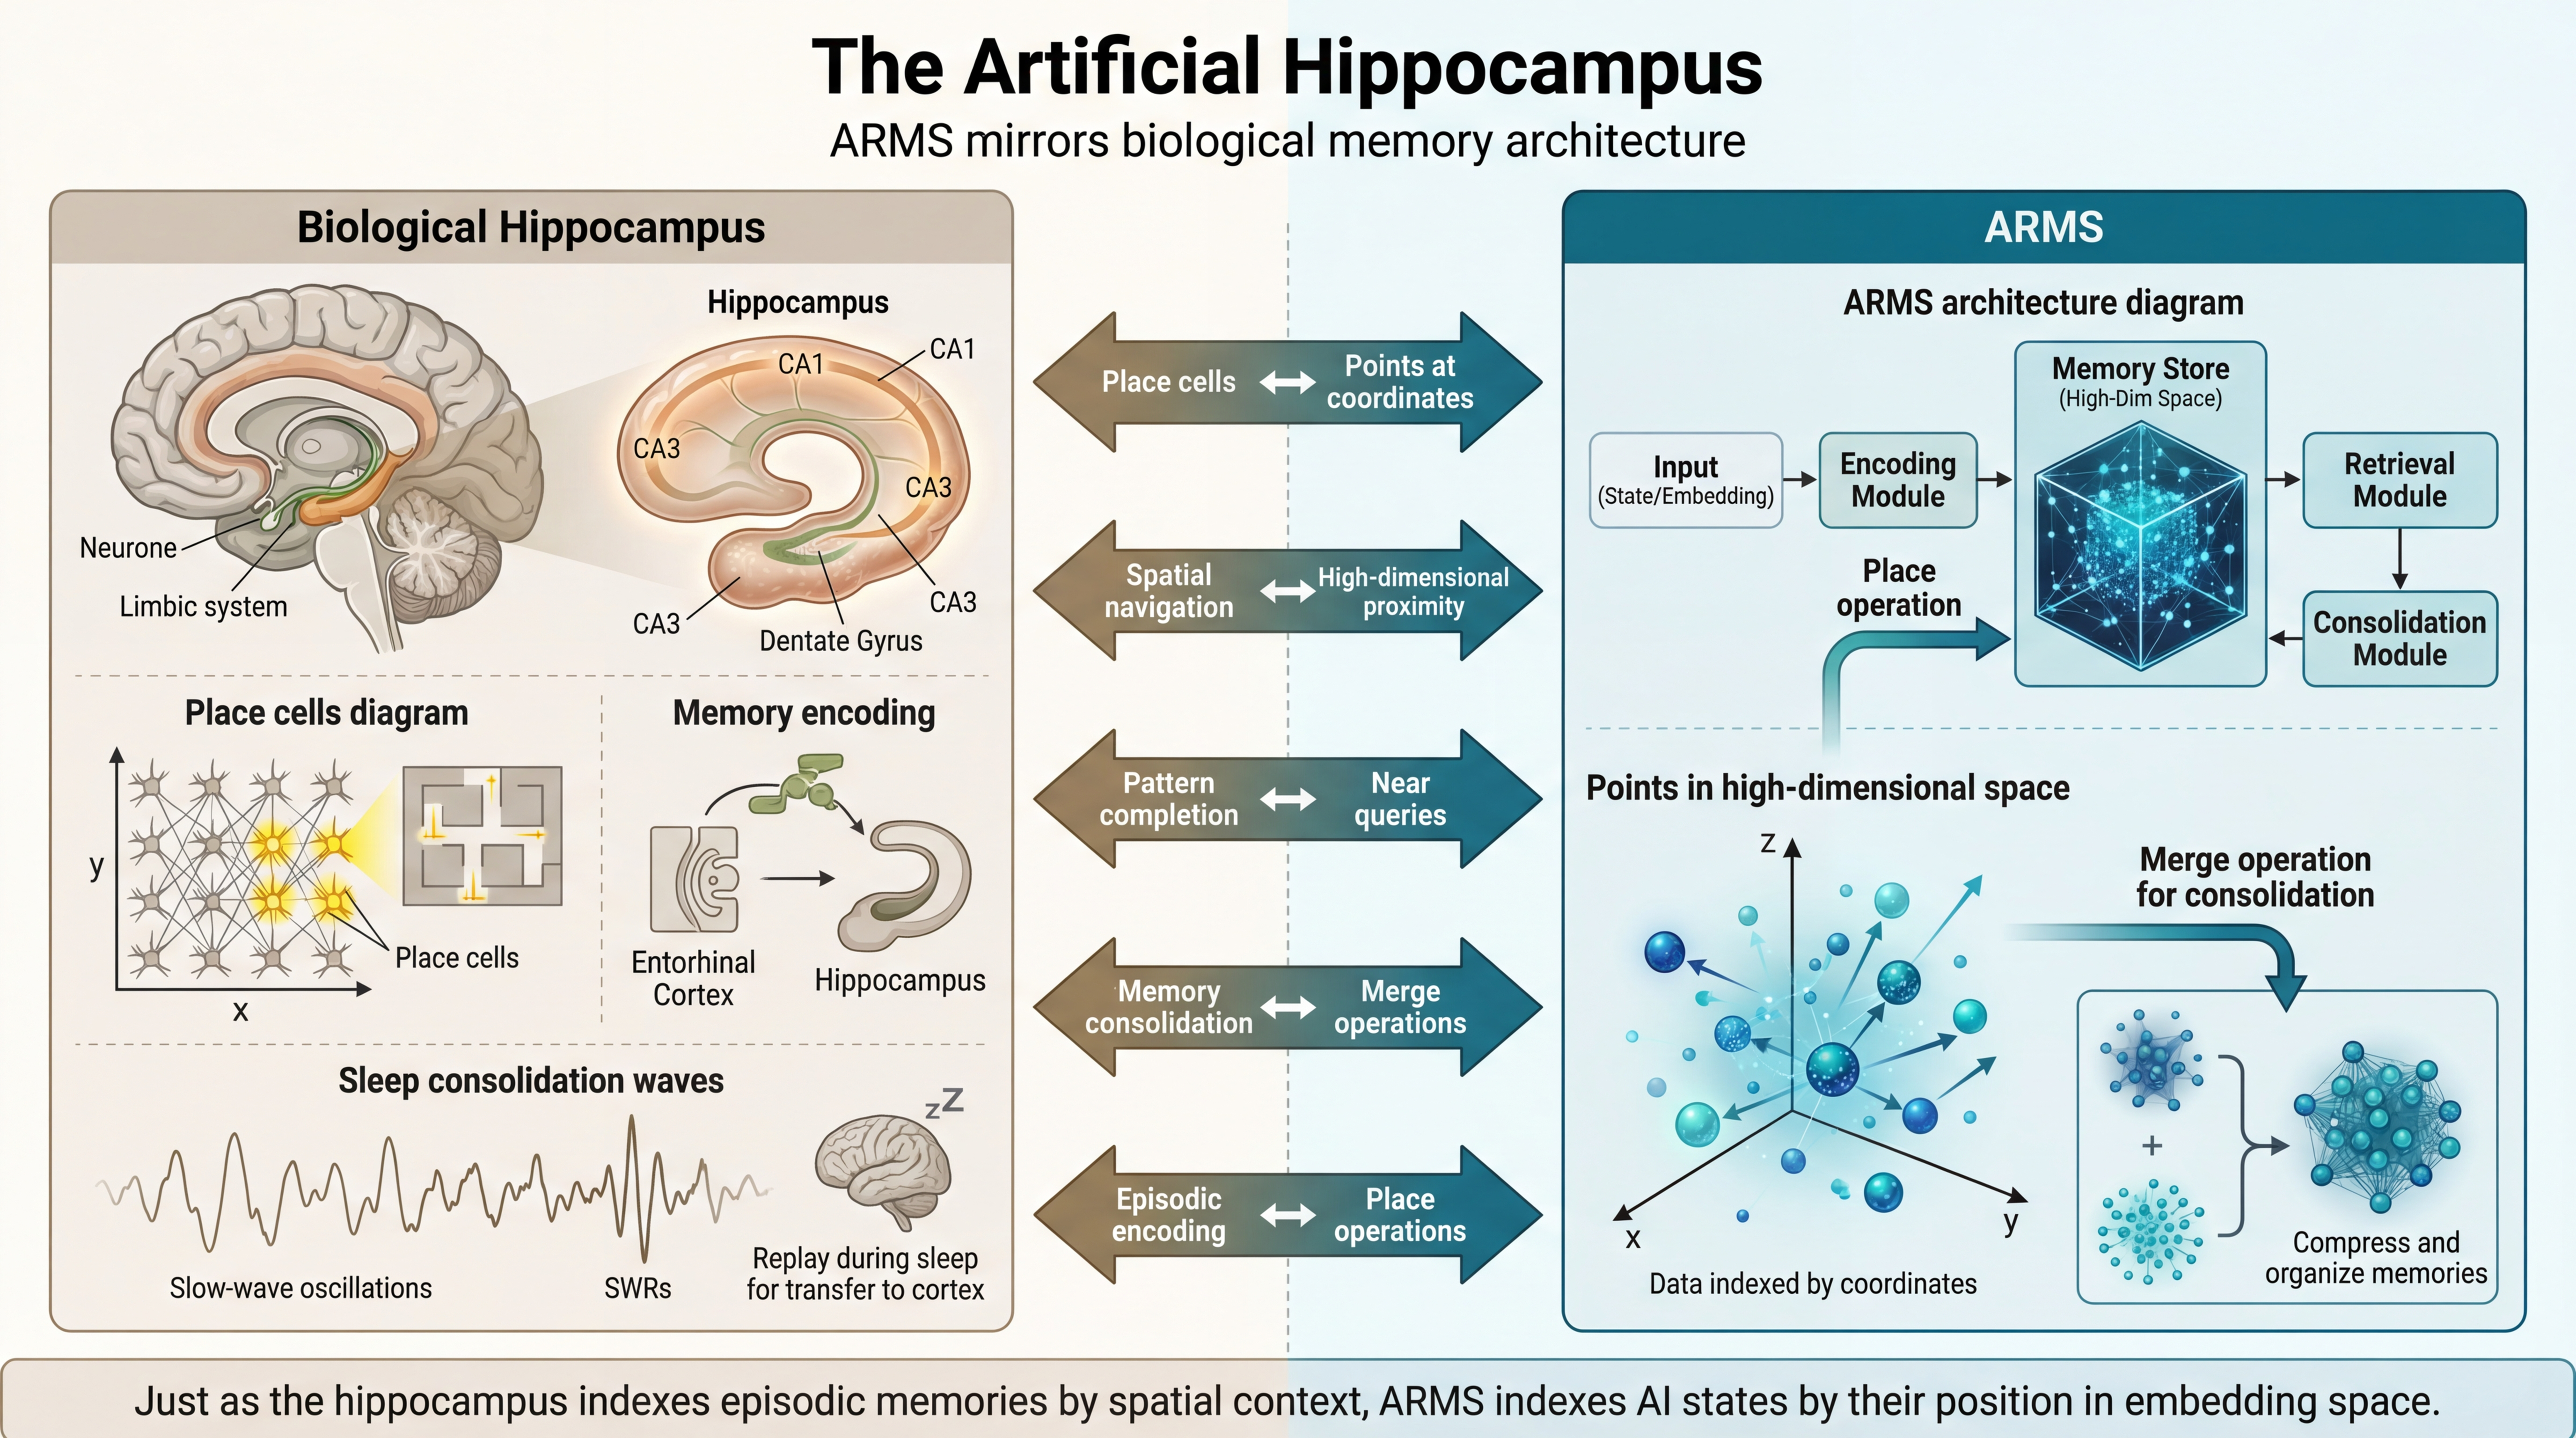
\includegraphics[width=0.85\textwidth]{fig05_hippocampus.jpg}
\caption{The hippocampus analogy: ARMS functions as an artificial hippocampus, enabling AI systems to form, consolidate, and retrieve episodic memories through spatial organization.}
\label{fig:hippocampus}
\end{figure}

\begin{table}[H]
\centering
\caption{Hippocampus vs ARMS.}
\label{tab:hippocampus}
\begin{tabular}{ll}
\toprule
\textbf{Hippocampus} & \textbf{ARMS} \\
\midrule
Encodes episodic memories & Stores attention states \\
Spatial navigation & High-dimensional proximity \\
Pattern completion & Near queries \\
Memory consolidation & Merge operations \\
Place cells & Points at coordinates \\
\bottomrule
\end{tabular}
\end{table}

% ----------------------------------------------------------------------------
\section{Implementation}
\label{sec:implementation}

ARMS is implemented in Rust for performance and safety, with Python bindings planned.

\subsection{Usage Example}

\begin{lstlisting}[language=Rust,caption={Complete ARMS usage example.}]
use arms_core::{Arms, ArmsConfig, Point, Blob};

// Create ARMS with 768 dimensions
let mut arms = Arms::new(ArmsConfig::new(768));

// Store embeddings
let embedding = Point::new(vec![0.1; 768]);
let id = arms.place(embedding, Blob::from_str("hello")).unwrap();

// Query by proximity
let query = Point::new(vec![0.1; 768]);
let neighbors = arms.near(&query, 10).unwrap();

// Get with data
let results = arms.near_with_data(&query, 5).unwrap();
for (point, score) in results {
    println!("{}: {}", point.blob.as_str().unwrap(), score);
}
\end{lstlisting}

\subsection{Performance}

With the flat index (exact search):

\begin{table}[H]
\centering
\caption{Flat index performance.}
\label{tab:performance}
\begin{tabular}{rrr}
\toprule
\textbf{Points} & \textbf{Dimensions} & \textbf{Query Time} \\
\midrule
1,000 & 768 & 0.3ms \\
10,000 & 768 & 3ms \\
100,000 & 768 & 30ms \\
\bottomrule
\end{tabular}
\end{table}

For large-scale deployments, the HAT index adapter provides $O(\log n)$ queries with 100\% recall on hierarchical data.

% ----------------------------------------------------------------------------
\section{Related Work}
\label{sec:related}

\textbf{Vector Databases}: Pinecone, Weaviate, Milvus, and Qdrant provide vector storage and retrieval. ARMS differs by providing a minimal primitive set and hexagonal architecture rather than a monolithic solution.

\textbf{Memory-Augmented Networks}: Neural Turing Machines and Differentiable Neural Computers use learned memory access. ARMS provides explicit, interpretable memory operations.

\textbf{RAG Systems}: Retrieval-Augmented Generation retrieves text for reprocessing. ARMS can store pre-computed attention states, avoiding recomputation.

\textbf{Embedding Stores}: LangChain, LlamaIndex provide embedding storage. ARMS provides lower-level primitives for building such systems.

% ----------------------------------------------------------------------------
\section{Future Work}
\label{sec:future}

\subsection{Planned Adapters}

\begin{itemize}
    \item \textbf{NVMe Storage}: Memory-mapped files for persistence
    \item \textbf{Distributed Storage}: Sharded across machines
    \item \textbf{GPU Index}: CUDA-accelerated similarity search
\end{itemize}

\subsection{Applications}

\begin{itemize}
    \item \textbf{LLM Memory}: Long-term episodic memory for chatbots
    \item \textbf{Agent State}: Persistent state for AI agents
    \item \textbf{Attention Caching}: Store and retrieve KV cache states
    \item \textbf{Multimodal Memory}: Unified space for text, image, audio embeddings
\end{itemize}

% ----------------------------------------------------------------------------
\section{Conclusion}
\label{sec:conclusion}

ARMS provides a minimal, principled foundation for AI memory systems. By reducing memory operations to five primitives and adopting a hexagonal architecture, ARMS enables:

\begin{enumerate}
    \item \textbf{Simplicity}: Five operations cover all memory needs
    \item \textbf{Flexibility}: Swap storage, index, and API independently
    \item \textbf{Performance}: Domain-specific adapters like HAT
    \item \textbf{Philosophy}: Position IS relationship
\end{enumerate}

ARMS functions as an artificial hippocampus for AI systems, enabling them to form, consolidate, and retrieve memories through spatial organization rather than explicit indexing.

% ----------------------------------------------------------------------------
\section*{Acknowledgments}

I thank the open-source Rust community for excellent tooling and the researchers whose work on memory-augmented networks inspired this architecture.

% ----------------------------------------------------------------------------
\bibliographystyle{plainnat}
\bibliography{refs}

% ----------------------------------------------------------------------------
\appendix

\section{Code Availability}
\label{app:code}

ARMS is available as open-source software:

\begin{itemize}
    \item \textbf{Rust crate}: \texttt{arms-core} on crates.io
    \item \textbf{HAT adapter}: \texttt{arms-hat} on crates.io
    \item \textbf{Repository}: \url{https://github.com/automate-capture/arms}
\end{itemize}

\end{document}
